\documentclass[11pt,letterpaper]{article}
\usepackage[lmargin=1in,rmargin=1in,bmargin=1in,tmargin=1in]{geometry}
\usepackage{style/quiz}
\usepackage{style/commands}

% -------------------
% Content
% -------------------
\begin{document}
\thispagestyle{title}


% Quiz 1
\quizsol \textit{True/False}: If $x \in A$ but $x \notin B$, then $x \notin A \cup B$. \pspace

\sol The statement is \textit{false}. Recall that if $S$ is a set, then $x \in S$ means that $x$ is an element of $S$. For example, suppose $S= \{ 1, 2, 3, 4, 5\}$. If $x= 1$, then $x \in S$. However, if $x= 9$ then $x$ is not in $S$, i.e. $x \notin S$. Recall also that $A \cup B$ is the set of elements that are either in $A$ or in $B$---including the possibility that it might be in both! Because $x \in A$, even though $x \notin B$, we know that $x \in A \cup B$ because $x$ is in $A$ or $B$---after all, it's in $A$! As a concrete example, take $A= \{ 1, 2, 3 \}$ and $B= \{ 2, 3, 4 \}$. Then we know that $A \cup B= \{ 1, 2, 3, 4 \}$. Now if $x= 1$, then $x \in A$ and $x \notin B$. But we can see that $x \in A \cup B$. \pvspace{1.5cm}



% Quiz 2
\quizsol \textit{True/False}: A person's salary at their first job is a function of their number of years of schooling. \pspace

\sol The statement is \textit{false}. Recall that a relation is a function if for each input, there is only one possible output, i.e. $f(x)$ is a function if given each $x$, there is one and only one possible output $f(x)$. In this example, we are wondering whether a person's income, $I$, is a function of their number of years of school, $n$. So is $I(n)$ a function? Then there would be one and only one possible output, i.e. salary, given some number of years of schooling. For instance, if $n= 4$~years (of high school, college, etc.), then the person's salary, $I(4)$, would have only one possible value. But we know that there are many people with the same number of years of schooling that have the same salary! For instance, there will be many people that graduate together (most having the same number of years of schooling) and will have widely varying salaries. Therefore, $I(n)$ cannot be a function, i.e. we cannot exactly predict someone's income from their number of years of school. However, one could try to perform statistical analysis on this problem, e.g. what does the \textit{average} person make if they have $n$ years of schooling. \pvspace{1.5cm}



% Quiz 3
\quizsol \textit{True/False}: A company is bulk ordering parts for their production line. The order is for $\$256,478.33$ and the processing company charges a $1$\% surcharge on an order. Therefore, the total they will be charged (before tax) for the goods is $\$256478.33(1.10) \approx \$282126.16$. \pspace

\sol The statement is \textit{false}. Because the company is charging a surcharge, the price is going up. We know the final bill will then be 1\%, i.e. we need to compute $\$256,478.33$ increased by 1\%. To compute a percentage increase/decrease of a number $N$ by $P\%$, we compute $N( 1 \pm P_d)$, where $N$ is the number, we choose `$+$' if we are computing an increase and `$-$' if we are computing a decrease, and $P_d$ is the percentage written as a decimal. In our case, writing $1$\% as a decimal, we have $0.01$. But then we have total $\$256\,478.33(1 + 0.01)= 256\,478.33(1.01) \approx \$259,043.11$.





\newpage





% Quiz 4
\quizsol \textit{True/False}: If there are three exams in a class. You received an 85\% on the first, 91\% on the second, and 78\% on the last. The exams are weighted such that the last is worth three times as much as the other two. Then your exam average is given by $85 \left( \frac{1}{5} \right) + 91 \left( \frac{1}{5} \right) + 78 \left( \frac{3}{5} \right)= 82\%$. \pspace

\sol The statement is \textit{true}. If this were an ordinary average, we could simply add up the grades and divide by the number of grades: $\frac{85\% + 91\% + 78\%}{3}= \frac{254\%}{3} \approx 84.7\%$. We can view this as a weighted average by algebraic manipulation and see that the weight is then one over the number of grades: $\frac{85\% + 91\% + 78\%}{3}= 85\% (\frac{1}{3}) + 91\% (\frac{1}{3}) + 78\% (\frac{1}{3}) \approx 28.33\% + 30.33\% + 26.0\% \approx 84.7\%$. In a weighted average, we add up each of the grades times their weight. For an ordinary average, this weight is simply $\frac{1}{n}$, where $n$ is the number of objects. Here, Exam~3 is worth three times as much as the other two. If we split the grade into five parts, the weights of Exam~1, Exam~2, and Exam~3 are $1/5$, $1/5$, and $3/5$, respectively. Then the exam average is $85\% (\frac{1}{5}) + 91\% (\frac{1}{5}) + 78\% (\frac{3}{5})= 17.0\% + 18.2\%.+ 46.8\%= 82\%$. \vfill



% Quiz 5
\quizsol \textit{True/False}: If~1 meter is 39.3701~inches, then to convert 5~m$^2$ to in$^2$, one computes $5 \cdot 39.3701 \approx 196.85$~in$^2$. \pspace

\sol The statement is \textit{false}. To convert this, we have\dots \par
	\begin{table}[!ht]
	\centering
	\begin{tabular}{c|c|c}
	5~m$^2$ & 39.3701~in & 39.3701~in \\ \hline
		     & 1~m 		  & 1~m 
	\end{tabular}
	$= 5 \cdot 39.3701 \text{ in} \cdot 39.3701 \text{ in}= (5 \cdot 39.3701^2) \text{ in}^2 \approx 7750.02 \text{ in}^2$
	\end{table}
As given, the individual only converted one of the units of meters to inches---neglecting to convert the other unit of meters to inches. So the given computation, $5 \cdot 39.3701 \approx 196.85$~in$^2$, was actually $5 \text{ m} \cdot 39.3701 \text{ in} \approx 196.85$~m~in, which does not have the correct units. \vfill



% Quiz 6
\quizsol \textit{True/False}: Suppose you have an hourly wage job. Then if you work twice as much for twice as much pay, you will make twice as much money. \pspace

\sol The statement is \textit{false}. Suppose that you made \$10/hr and work 8~hours a week. Then you make \$10/hr $\cdot$ 8~hours $=$ \$80. Now if you double each of those, you make \$20/hr and work 16~hours per week. But then you make \$20/hr $\cdot$ 16~hours $=$ \$320, which is four times the amount---not double the amount. Generally, suppose you make $r$ dollars an hour and work $h$ hours a week. Then you make $P= r \cdot h$ dollars a week. Now suppose you double your pay and hours a week. Then you make $(2r)(2h)= (2 \cdot 2)(rh)= 4P$ dollars a week, which is four times the amount---not double. \vfill





\newpage





% Quiz 7
\quizsol \textit{True/False}: If you travel 6~mi west and 10~mi south, then you have traveled approximately 11.7~mi from your original location---as the crow flies. \pspace

\sol The statement is \textit{true}. The distance `as the crow flies', is the straight line distance from one point to another. Drawing this out, we have\dots
	\[
	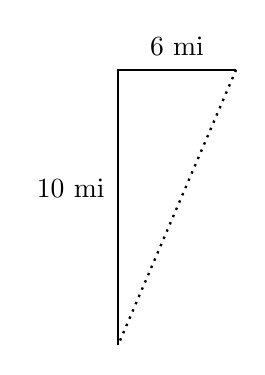
\begin{tikzpicture}
	\draw[line width= 0.03cm,black] (0,0) -- (-1.5,0) -- (-1.5,-3.5);
	\node at (-0.75,0.3) {$6$~mi};
	\node at (-2.1,-1.5) {$10$~mi};
	\draw[line width= 0.03cm,black,dotted] (0,0) -- (-1.5,-3.5);
	\end{tikzpicture}
	\] 
The distance we want is the dotted line---the hypotenuse of the triangle sketched above. But by the Pythagorean Theorem, we have\dots
	\[
	d= \sqrt{a^2 + b^2}= \sqrt{(6 \text{ mi})^2 + (10 \text{ mi})^2}= \sqrt{36 \text{ mi}^2 + 100 \text{ mi}^2}= \sqrt{136 \text{ mi}^2} \approx 11.66 \text{ mi}^2.
	\] \pvspace{1.5cm}



% Quiz 8
\quizsol \textit{True/False}: `Any' function which has a constant rate of change can be represented by a linear function. \pspace

\sol The statement is \textit{true}. Suppose the rate of change were 5 and the current value is 2. After one step in time, the value is $2 + 1(5)= 2 + 5= 7$. After another step in time, the value is $7 + 5= 12$, or $2 + 2(5)= 2 + 10= 12$. Generally, after $n$ steps, the value is $2 + n \cdot 5= 5n + 2$, which is a linear function. Generally, if we start with initial value $y_0$ and have a constant rate of change $m$, after $x$ steps, we have $y= y_0 + x \cdot m= mx + y_0$. This is a linear function with $y= y$, $x= x$, $m= m$, and $b= y_0$. But then we see that `any' function which changes at a constant rate is a linear function. We know that a linear function $y= mx + b$ has a constant rate of change---the slope $m$. Therefore, a function is linear if and only if it has a constant rate of change. 









\end{document}